\begin{figure*}[t]
    \centering
    \begin{subfigure}[b]{0.5\textwidth}
        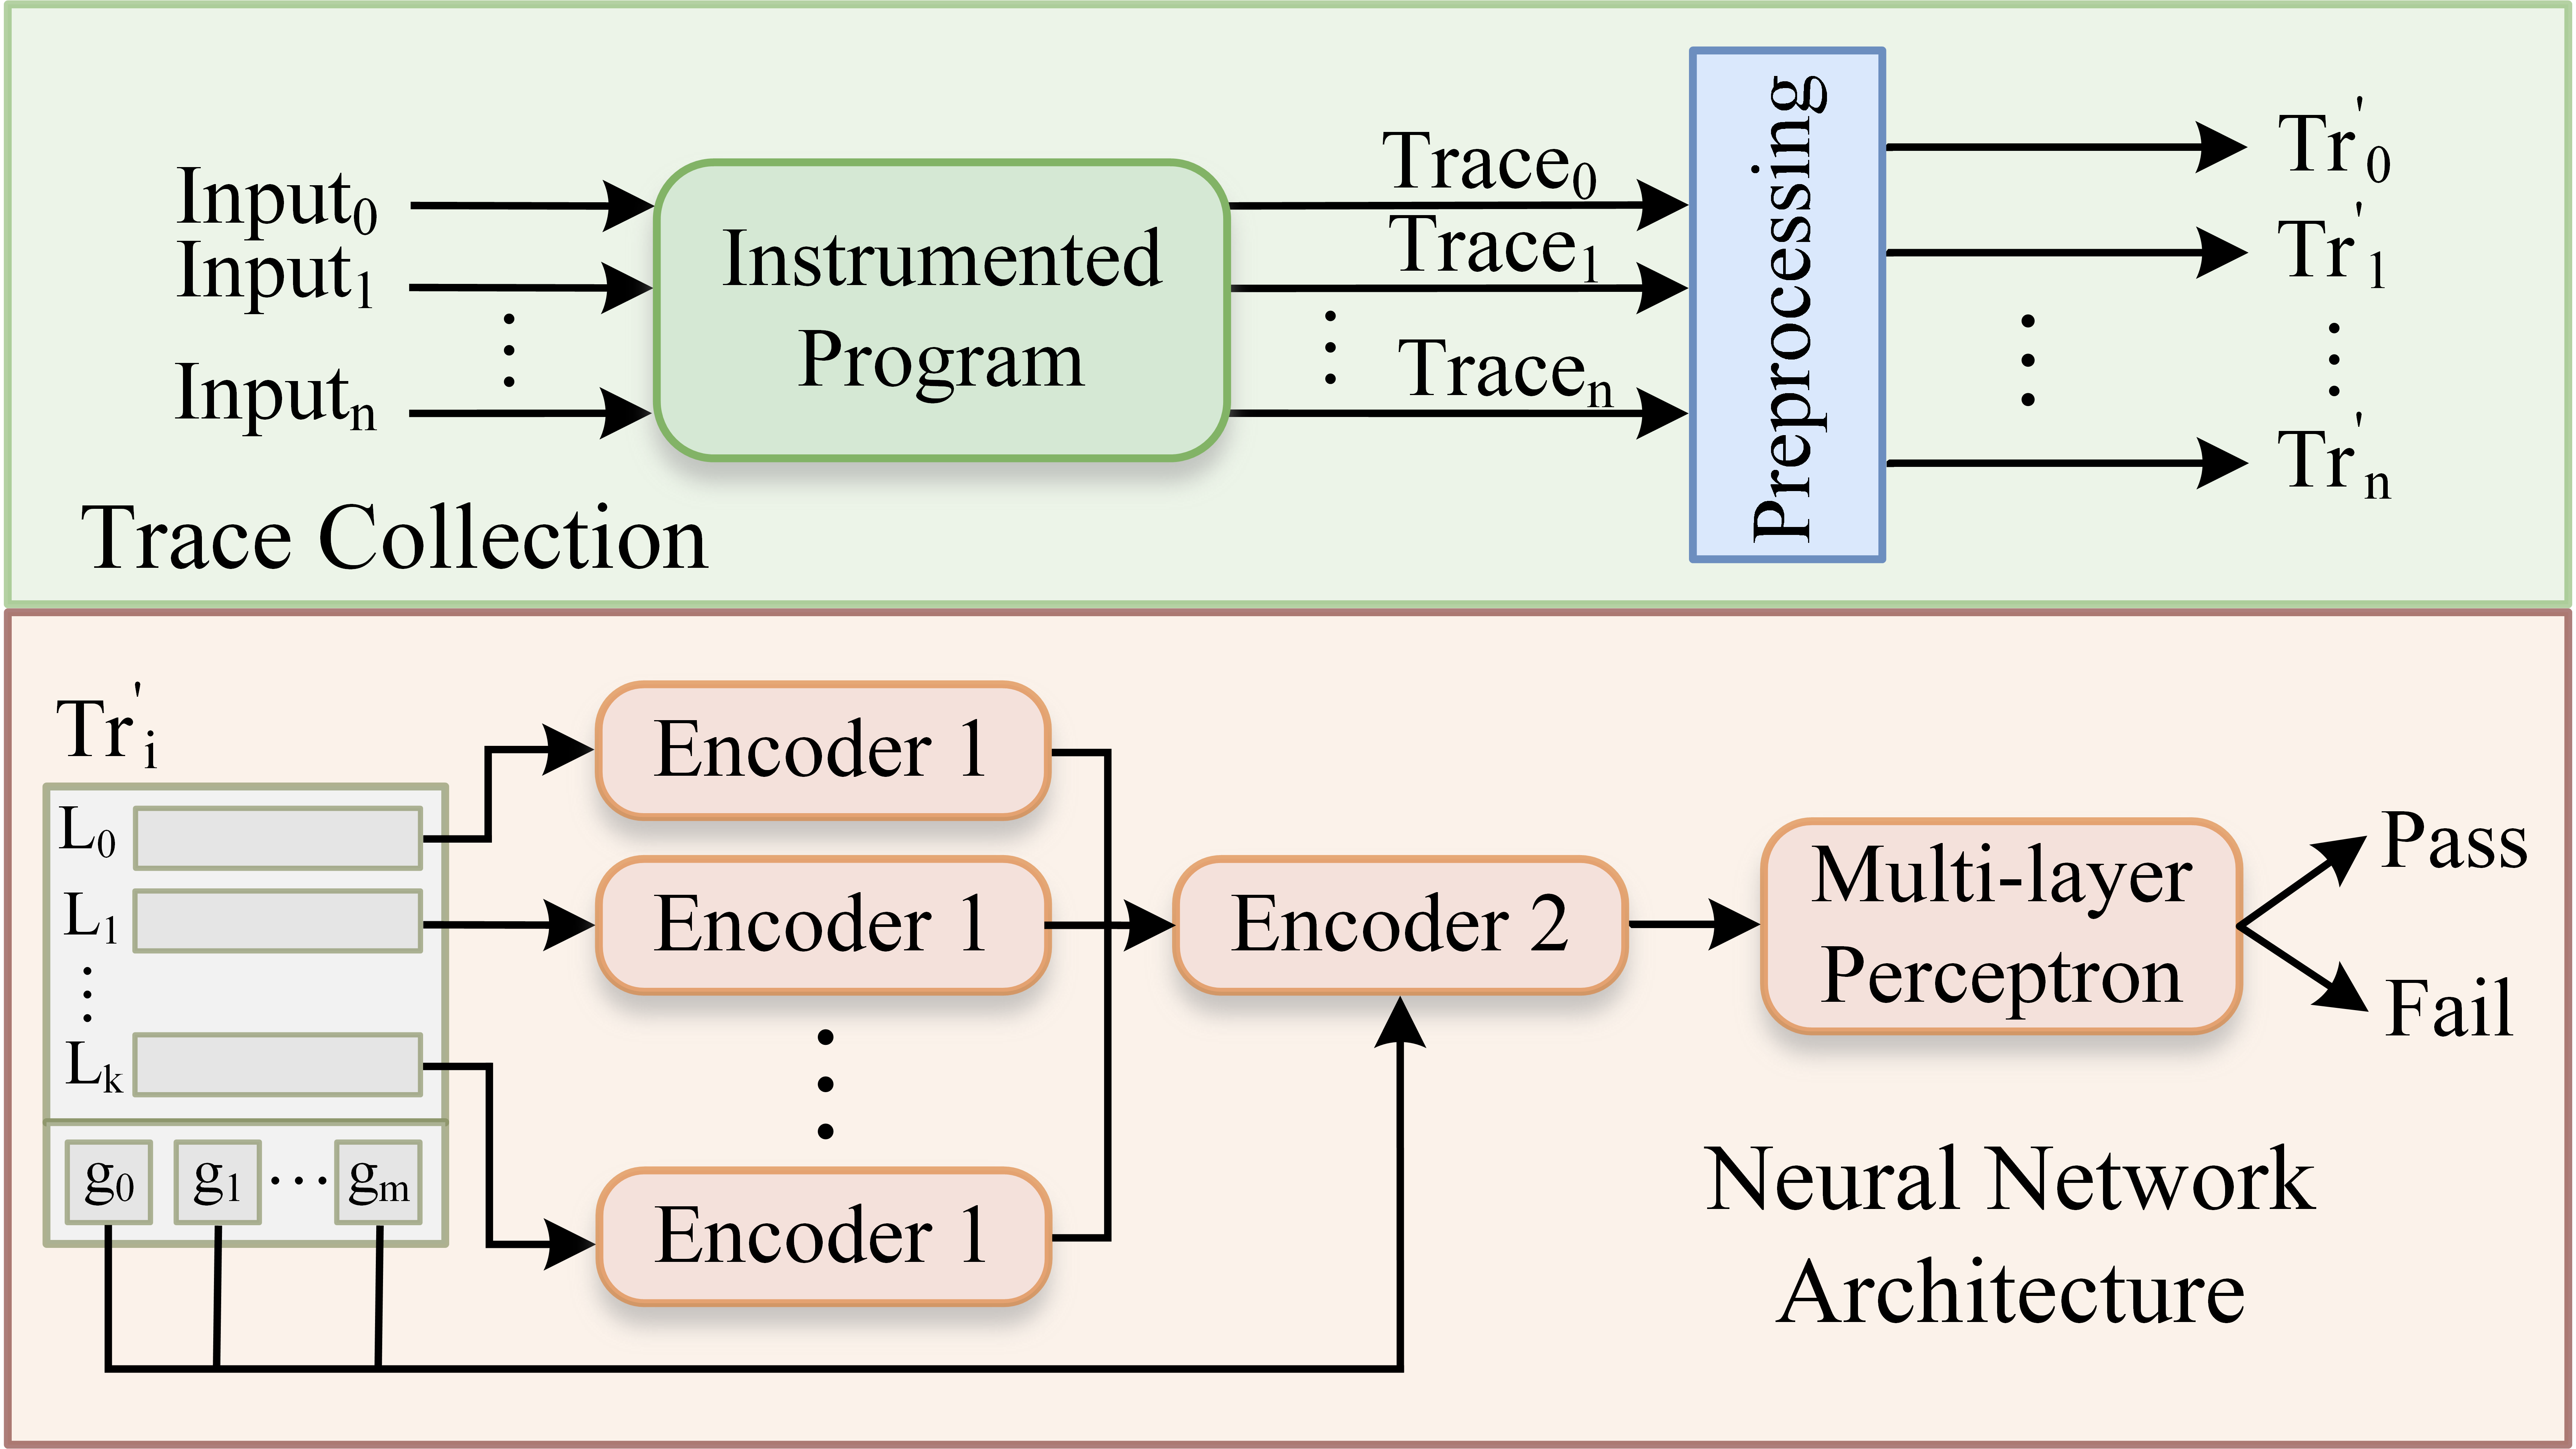
\includegraphics[scale=0.88]{../../figures/pipeline.png} %1.071
    %\vspace{-6pt}
    \caption{Gathering traces, encoding them, and using NNs to classify them.}
        %\vspace{0.5cm}
        \label{fig:pipeline}
    \end{subfigure}~~
    \centering
    \begin{subfigure}[b]{0.5\textwidth}
        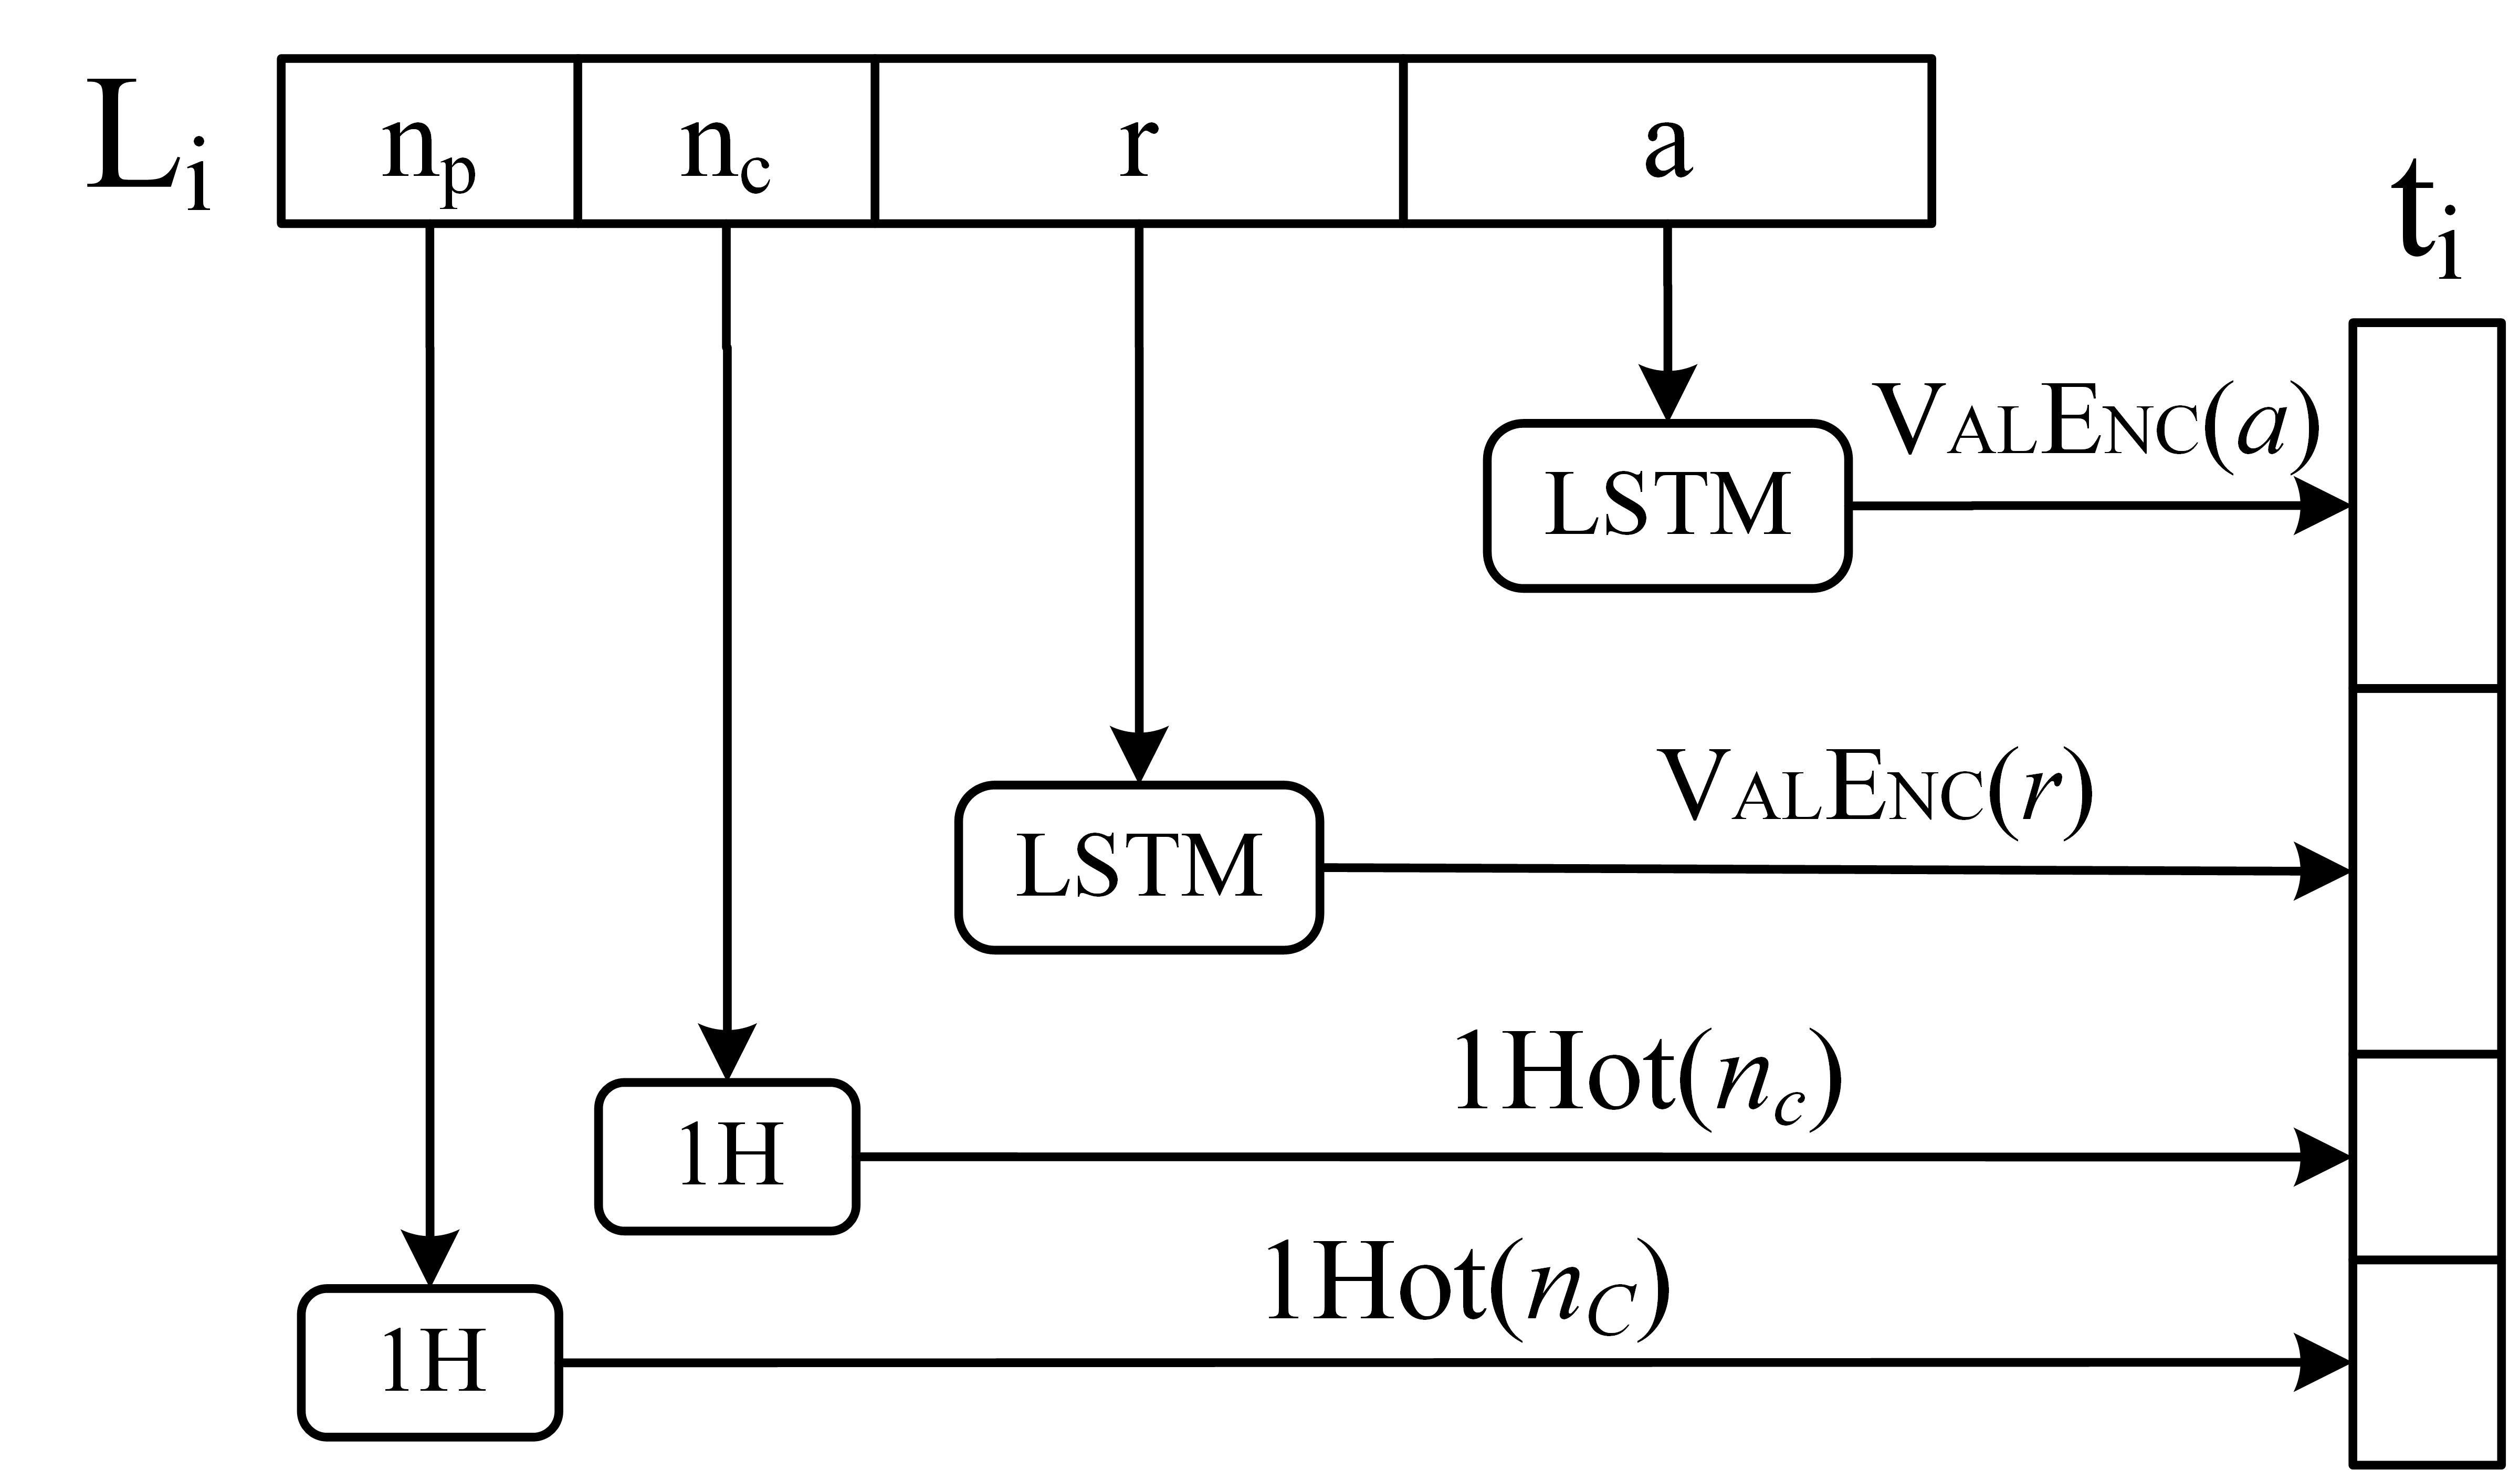
\includegraphics[scale=0.8]{../../figures/encoder_1.png} %1.0
%        \vspace{0.25cm}
%\vspace{10pt}
        \caption{\texttt{Encoder 1} representing a single line in a trace as a vector containing function caller, callee names, arguments and return values. }
%        \vspace{0.25cm}
        \label{fig:encoder-1}
    \end{subfigure}
 \vspace{-10pt}
 \caption{High-level architecture of our approach and \texttt{Encoder 1} description.}
    \vspace{-4pt}
%    \Description[High-level architecture of our approach and \texttt{Encoder 1} description.]{}
\end{figure*}
\iffalse
\begin{figure}[ht!]
    \centering
    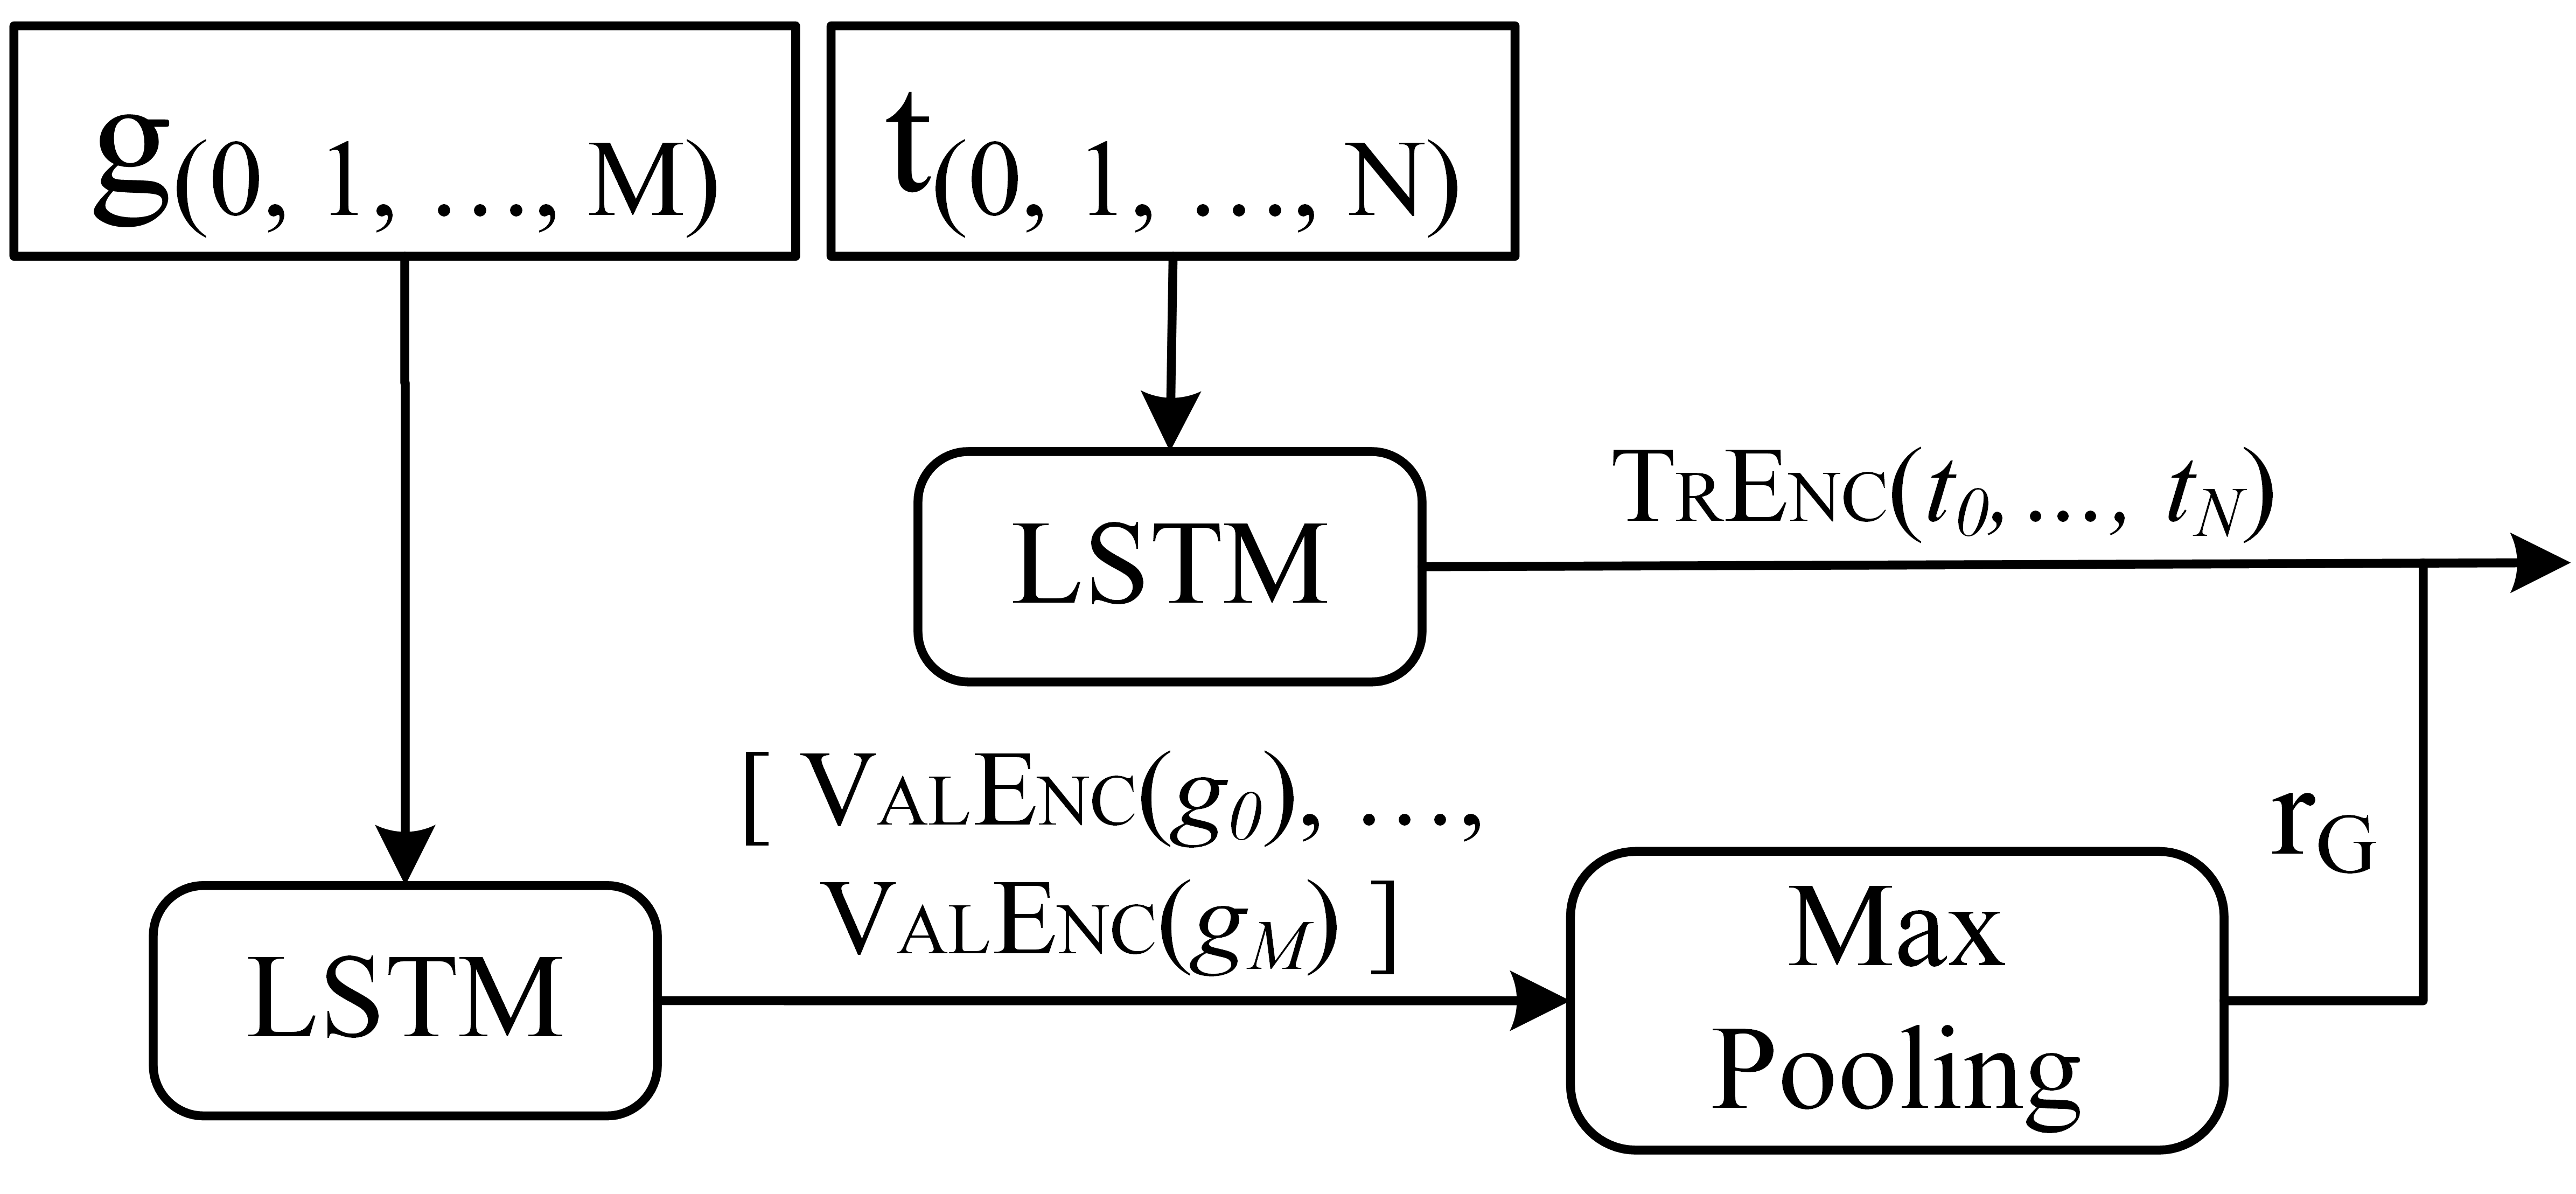
\includegraphics[scale=0.8]{../figures/encoder_2.png}
    \caption{\texttt{Encoder 2} representing a sequence of trace lines and global state as a single vector.}
    %\vspace{-20pt}
    \label{fig:encoder-2}
    \vspace{-10pt}
    %\Description[\texttt{Encoder 2} representing a sequence of trace lines and global state as a single vector.]
\end{figure}
\fi
\iffalse
\begin{figure}[ht!]
	\centering
	\includegraphics[scale=0.3]{../figures/mutation.png}
	\caption{Labelling test executions by matching actual and expected behavior.}
	%\vspace{-20pt}
	\label{fig:labelling}
	\vspace{-10pt}
	%\Description[\texttt{Encoder 2} representing a sequence of trace lines and global state as a single vector.]
\end{figure}
\fi
Our approach for building an automated test oracle for classifying execution traces has the following steps,
\begin{description}[itemsep = 0pt, topsep = 0pt, partopsep=0pt]
 \item[Step 1:] Instrument the PUT to gather traces when executing the test inputs.
 \item[Step 2:] Preprocess the traces to prune unnecessary information.
 \item[Step 3:] Encode the preprocessed traces into vectors that can be accepted by the neural network.
 \item[Step 4:] Design a NN model that takes as input an encoded trace, and outputs a verdict of pass or fail for that trace.
\end{description}
Figure~\ref{fig:pipeline} illustrates the steps in our approach, with the bottom half of the figure depicting steps 3 and 4 for any given preprocessed trace from step 2.
We discuss each of the steps in the rest of this Section.
%A high level view of our system is shown in figure~\ref{fig:pipeline}.
% \begin{itemize}
% \item The runtime instrumentation framework.
% \item The data preprocessing tool.
% \item The encoding of the traces.
% \item The architecture of the neural network.
% \end{itemize}

\subsection{Instrument and Gather Traces}
\label{sec:instrument}
For every test input executed through the PUT, we aim to collect an execution trace as a sequence of method invocations, where we capture the name of the method being called, values and data types of parameters, return values and their types, and, finally, the name of the parent method in the call graph. We find gathering further information, eg. updates to local variables within each method, incurs a significant overhead and is difficult to scale to large programs. %information in traces incurs a significant overhead for large programs.
To gather this information we use the middleware of LLVM~\cite{LLVMoriginal} and instrument the intermediate representation (IR) of programs.
This allows our implementation to be language-agnostic. LLVM provides front-end support for multiple programming languages, such as C/C++, CUDA, Haskell, Swift, Rust among others, along with numerous libraries for optimisation and code generation.
%\item The IR provides a detailed, but high-level, view of the program interactions with the memory and data type initialization, thus potentially exposing information about defects that would not be easily observed in the high-level code.
%\item The high-level constructs and features of the programming language are simplified and unified, removing syntactic sugar that induces unneeded sparsity to the data
%while allowing us to instrument these programs more easily.


% TODO: Find better symbols!
\newcommand{\callerName}{\ensuremath{n_p}\xspace}
\newcommand{\calleeName}{\ensuremath{n_c}\xspace}
\newcommand{\rVal}{\ensuremath{r}\xspace}
\newcommand{\argVals}{\ensuremath{a}\xspace}
%\ajitha{2 sentences on LLVM IR ..}
To perform the instrumentation, we traverse the PUT, visiting each method. Every time a method invocation is identified, code is injected to trace the caller-callee pair, the arguments and the return values. At the end of the program, code is inserted to write the trace information to the output.

Each trace contains a sequence of method invocations. This sequence comprises multiple lines, each line being a tuple $(\callerName, \calleeName, \rVal, \argVals)$ that represents a single method invocation within it having:

\begin{itemize}
\item The names of the caller (parent) \callerName and called \calleeName functions.
\item Return values \rVal of the call, if any.%\ajitha{Types?? After bullets}
\item Arguments passed \argVals, if any.
\end{itemize}
The order of trace lines or method invocations is the order in which the methods complete and return to the calling point. We support all variable types including primitive types (such as \texttt{int, float, char, bool}), composite data types (such as structs, classes, arrays) defined by a user or library,  and pointers for return and argument values. Structs and classes are associated with a sequence of values for their internal fields. We instrument these data structures in a depth first fashion, until all primitive types are traced. For pointers, we monitor the values they refer to.  %\foivos{anything special for recording values of pointers?}


%\textcolor{blue}{The types of the return and argument values can be a primitive, user or library-defined types in the high-level source code. As for class objects, they are represented as a sequence of their %underlying primitive fields. This happens by instrumenting fields in a DFS manner, until all primitive types are traced.}

%\ajitha{How is global state represented within the trace? Below}

%\textcolor{blue}{Within the second section of the trace, each line contains the value of one global variable before program termination. This line might contain a single number (if the respective variable is a primitive type), or a sequence of values (if the variable is a class object with multiple internal fields). }

\subsection{Training Set}
\label{sec:labelled-traces}
We execute the instrumented program with each test input in the test suite to gather a set of traces. A subset of the traces is labelled and used in training the classification model. To label the traces as pass or fail, we compare actual outputs through the PUT with expected outputs provided by a reference program or the specifications. %, as shown in figure~\ref{fig:labelling}.
Section~\ref{sec:labelling-traces} discusses how we label traces for the subject programs in our experiment. 
It is worth noting that in our approach, the developer will only need to provide expected outputs for a \emph{small proportion of tests rather than the whole test suite}. %In current practices, the developer or tester provides expected outputs for the whole test suite which is considerably more effort than the 15\% we require. 
In the absence of expected output in tests, how will tests be labelled is a common question. Answering this question will depend on what is currently being done by the developer or organisation for classifying tests as pass or fail. Our approach will entail applying the same practice to labelling, albeit to a significantly smaller proportion of tests.    % will rely on the existing test classification practice used by the organisation to label a small proportion of tests.
%The advantage with our technique is that only a small proportion of the traces will need to be labelled as opposed to all the tests which is the case for current practices.
%
%If the tests do not specify expected outputs, then the relevant technique that the develper or organisation currently relies on for classifying tests can be used to label the traces. This relevant technique may be manual inspection, a golden reference model or a developer or expert would have to manually label the traces used in training, which is a small proportion of the total traces.  Reuiring a small proportion of traces to be labelled is \emph{not} a limitation of our approach
\iffalse
\textcolor{red}{We also find that some programs are only accompanied by passing tests, whereas both classes} are needed in the training set.
To generate failing tests, we keep the original program as a reference for the expected outputs and we use common bugs to mutate it. If a test's output deviates from the expected output, it is labelled as failing, otherwise passing. We gather all execution traces by running all tests through the mutated program.
We apply the following mutations representing some common bug patterns~\cite{jia2011analysis, pradel2018deepbugs}: %that are most applicable to the code structure and syntax for the subject programs in our experiment:
\begin{enumerate}[itemsep = 0pt, topsep = 0pt, partopsep=0pt]
	\item Logical connector replacement applied to \{$\&\&, ||, !$\}.
	\item Relational operator replacement applied to \\ \{$<, > , ==, <=, >=, !=$\}.
	\item Argument swapping in function calls.
	\item Scalar variable replacement.
	\item Loop boundary value replacement.
\end{enumerate}
\fi
To avoid data leakage in our experiment in Section~\ref{sec:experiment}, we ensure that expected output is removed from the traces. We also remove exceptions, assertions and any other information in the program or test code that may act as a test oracle. This is further discussed in Section~\ref{sec:subj-programs}. %\foivos{This is what we originally mentioned for data leakage}
%
%We assume that the original program is correct and, therefore, the traces gathered from it are labeled as passing. To produce failing traces, random mutations are applied to the %original IR of the program. In this work, we consider swapping binary operators, changing loop boundaries, inverting Boolean statements or swapping the arguments in a function %call. Each mutation generates a single set of failing traces.
%
%Even though the test cases of the projects we study, are using assertions to compare the computed with the expected output
%The test cases of the projects we study, are using assertions to compare the computed with the expected output of each test input. However, it is important to note that, before instrumentation, we have removed these assertions or any other kind of information that could betray the validity of the output. The desired behavior of our architecture is to understand how the control flow is correlated with the input, output and the correctness of a program, instead of overfitting on a binary state, which is at the end of the trace and represents if the test passed or failed.

\subsection{Preprocessing}
The execution traces gathered with our approach include information on methods declared in external libraries, called during the linking phase. To keep the length of the traces tractable and relevant, we preprocess the traces to only keep trace lines for methods that are defined within the module, and remove trace lines for declared functions that are not defined, but simply linked to later.
%to only keep trace lines for methods and implementations defined by the \textcolor{red}{user} \foivos{user defined methods are a subset of the defined functions in a IR module. Others are functions from locally-based header files included, or methods not explicitly specified by the user, e.g. constructors for the containers they use. They are as well important} and remove
%trace lines for declared functions from external libraries.
%The execution traces collected can be quite long. Due to well-known limitations of neural networks with long sequences, it is necessary to preprocess the traces to reduce their length. The length of the traces is large, predominantly due to the fact that, on compiler level, many function are invoked to construct objects at the beginning of each program. For example, invoking a simple C++ function that only initializes and returns a vector, can produce an execution trace of 50 lines. To alleviate this issue, function calls that occur before a certain point in the trace are rejected. We choose that point to be the first function call that directs the control flow to the function (or the first function among many) under test \foivos{this sentence is too cryptic!}. This approach is correct since before reaching the tested function, no differences relative to potential bugs can be observed.
%\foivos{The above paragraph is very hard to understand, what are you trying to say? What trace lines are disregarded?}

For method invocations within loops, a new trace line is created for each invocation of the same method within the loop. For loops with large numbers of iterations, this can lead to redundancy when the method is invoked with similar arguments and return values. We address this potential redundancy issue by applying average pooling to trace lines with identical caller-callee methods within loops.
%Furthermore, function calls inside lengthy loops can lead to an unwanted increase of trace length. In most cases, functions called inside loops receive similar arguments and return similar values. To summarize information from identical function calls in a sequence, average pooling is applied to these lines. If the number of consecutive identical sequences of function calls surpass a threshold, then pooling is applied to this sequence. As an example, if 50 sequential function calls with identical sets of caller-callee functions are found into a trace, they will be summarized as 10 averaged lines by selecting pooling kernel and stride equal to 5, if pooling is activated. Selecting the length of the pooling kernel, as well as the threshold which triggers it, is specified individually for each application, after experimenting with the original traces.


% excluded declared functions which are typically called during the linking phase. These declared functions are external library functions, like methods for STL containers and functions in the BOOST library.
%- why?
% Too expensive to monitor everything, menanigful information will be lost, you assume library functions work correctly
% only trace method invocations that are defined and implemented within the PUT.
%\foivos{I have my doubts about the former paragraph. We might create more questions than explain something actually meaningful. Also it is not that this pooling is so important to the preprocessing. It is rather used in 1-2 occasions}

 % \foivos{What is avg pooling in this setting?} \miltos{Well, the idea is: If you have a function call inside a loop, then you will find in the trace, X consecutive lines being exactly the same, or almost the same, differing just a bit in their arguments (most of the times because of loop increment). So, for example, if the preprocessor found 50 consecutive function calls, with the same caller-callee pair, it would apply avg pooling with kernel=stride= say 10, and you would end up with 5 averaged lines, instead of 50.} \foivos{Then explain this in the text and delete these TODOs}

\subsection{Neural Network Model}
\label{sec:NN-model}
\newcommand{\valEncoder}{\textsc{ValEnc}\xspace}
\newcommand{\traceEncoder}{\textsc{TrEnc}\xspace}
\newcommand{\traceClassifier}{\textsc{TraceClassifier}\xspace}
In this step, we perform the crucial task of designing a neural network that learns to classify the pre-processed traces as passing or failing.
Shape and size of the input traces vary widely, and this presents a challenge when designing a NN that accepts fixed length vectors summarizing the traces.
%The challenge arises from the widely varying shape and size of the input traces. Although this is a standard classification problem, the shape and size of each trace differs widely.
To address this, our network comprises three components that are trained jointly and end-to-end: 1. a \valEncoder that encodes values (such as the values of arguments and return values) into $D_V$-dimensional distributed vector representations, shown within \texttt{Encoder 1} in Figure~\ref{fig:encoder-1}, 2. a \traceEncoder that encodes variable-sized traces into a single $D_T$-dimensional vector, shown as \texttt{LSTM} in Figure~\ref{fig:pipeline}, and finally, 3. a \traceClassifier that accepts the trace representation for state and predicts whether the trace is passing or failing. The \texttt{Multi-layer Perceptron} in Figure~\ref{fig:pipeline} represents the \traceClassifier.  We describe each component in detail in the rest of this section.

\textbf{Encoding Values}
Values within the trace provide useful indications about classifying a trace. % and therefore, we need to incorporate information about those values in a way that our neural network can learn from patterns within them.
However, values --- such as ints, structs, and floats --- vary widely in shape and size. We, therefore, design models that can summarize variable-sized sequences into fixed-length representations. In the machine learning literature, we predominantly find three kinds of models that can achieve this: recurrent neural networks (RNNs), 1D convolutional neural networks (CNN) and transformers. In this work, we employ LSTMs~\cite{hochreiter1997long} --- a commonly used flavour of RNNs. Testing other models is left as future work. At a high-level RNNs are recurrent functions that accept a vector $\mathbf{h}_t$ of the current state and an input vector $\mathbf{x}_t$ and compute a new state vector $\mathbf{h}_{t+1}=RNN(\mathbf{x}_t, \mathbf{h}_t)$ which ``summarizes'' the sequence of inputs up to time $t$. A special initial state $\mathbf{h}_0$ is used at $t=0$.

To encode a value $v$, we decompose it into a sequence of primitives $v=[p_0, p_1, ...]$ (integers, floats, characters, etc.). Each primitive $p_i$ is then represented as a binary vector $\mathbf{b}_i=e(p_i)$ containing its bit representation padded to the largest primitive data type of the task. For example, if \texttt{int64} is the largest primitive then all $\mathbf{b}_i$s have dimensionality of 64. This allows us to represent all values (integers, floats, strings, structs, pointers, etc.) as a unified sequence of binary vectors. We encode $v$ into a $D_V$-dimensional vector by computing
\begin{align*}
	\valEncoder(v) = LSTM_{v}(e(p_L)_L, \valEncoder([p_0, p_1, ..., p_{L-1}])),
\end{align*}
where $LSTM_{v}$ is the LSTM that sequentially encodes the $\mathbf{b}_i$s. Note that we use the same \valEncoder for encoding arguments and return values, as seen in Figure~\ref{fig:encoder-1}. The intuition behind this approach is that the bits of each primitive can contain valuable information. For example, the bits corresponding to the exponent range of a float can provide information about the order of magnitude of the represented number, which in turn may be able to discriminate between passing and failing traces.

\textbf{Representing a Single Trace Line}
\newcommand{\OneHot}{\textsc{1Hot}\xspace}
Armed with a neural network component that encodes values, we can now represent a single line $(\callerName, \calleeName, \rVal, \argVals)$ of the trace. To do this, we use \valEncoder to encode the arguments \argVals and the return value \rVal. We concatenate these representations along with one-hot representations of the caller and callee identities, as shown in Figure~\ref{fig:encoder-1}. Specifically,
the vector encoding $\mathbf{t_i}$ of the $i$th trace line is the concatenation
\begin{align*}
	\mathbf{t_i} = \left[ \valEncoder(\argVals), \valEncoder(\rVal), \OneHot(\callerName), \OneHot(\calleeName) \right],
\end{align*}
where \OneHot is a function that takes as input the names of the parent or called methods and returns a one-hot vector that uniquely encodes that method name. For methods that are rare (appear fewer than $k_{min}$ times) in our data, \OneHot collapses them to a single special Unknown (UNK) name. This is similar to other machine learning and natural language processing models and reduces sparsity often improving generalization.
The resulting vector $\mathbf{t_i}$ has size $2D_V+2k$ where $k$ is the size of each one-hot vector.

\textbf{Encoding Traces}
Now that we have built a neural network component that encodes single lines within a trace, we design \traceEncoder that accepts a sequence of trace line representations $\mathbf{t}_0 ... \mathbf{t}_N$ and summarizes them into a single $D_T$-dimensional vector. We use an LSTM with a hidden size $D_T$, and thus
\begin{align*}
	\traceEncoder(\mathbf{t}_0 ... \mathbf{t}_N) = LSTM_{tr}\left(\mathbf{t_N}, \traceEncoder(\mathbf{t}_0 ... \mathbf{t}_{N-1}) \right),
\end{align*}
where $LSTM_{tr}()$ is an LSTM network that summarizes the trace line representations. %Figure~\ref{fig:encoder-2} shows \traceEncoder along with global state encoding.

\iffalse
\textcolor{red}{\textbf{Encoding Global State} We encode the final values of global variables in each trace. %The global state can provide valuable information for trace classification and thus we also encode the values within the global state.
Assuming global variables $g_0, ..., g_M$, we first encode them using \valEncoder and then summarize the global state into a single vector
\begin{align*}
\mathbf{r}_G = \textsc{Pool}(\valEncoder(g_0), ... \valEncoder(g_M)),
\end{align*}
where \textsc{Pool} is a permutation-invariant pooling function and $\mathbf{r}_G$ is a $D_V$-sized vector. In this work, we use max pooling (i.e. element-wise maximum). Note that the permutation invariance is a necessary design requirement since the representation of the global state should be invariant to the ordering of the global variables. Figure~\ref{fig:encoder-2} shows \traceEncoder along with global state encoding.}
\fi

\textbf{Classifying Traces}
%Our task is to classify a trace into either passing or failing.
With the neural network components described so far we have managed to encode traces into fixed length vector representations. The final step is to use those computed representations to make a classification decision. We treat failing traces as the positive class and passing traces as the negative class since detecting failing runs is of more interest in testing.  We compute the probability that a trace is failing as
\begin{align*}
	P(\textsf{fail}) = \traceClassifier([\traceEncoder(\mathbf{t}_0 ... \mathbf{t}_N)]),
\end{align*}
where the input of \traceClassifier is the output vector of \traceEncoder. Our implementation of \traceClassifier is a multilayer perceptron (MLP) with sigmoid non-linearities and a single output, which can be viewed as the probability that the trace is a failing trace. It follows that $P(\textsf{pass})=1-P(\textsf{fail})$.

\textbf{Training and Implementation Details}
We train our network end-to-end in a supervised fashion, minimizing the binary cross entropy loss. All network parameters (parameters of $LSTM_v$ and $LSTM_{tr}$ and parameters of the MLP) are initialized with random noise.
For all the runs on our network we use $D_V=128$, $D_T=256$. The \traceClassifier is an MLP with 3 hidden layers of size 256, 128 and 64.
We use the Adam optimizer~\cite{AdamOptimizer} with a learning rate of $10e-5$. 

For our subject programs, we find the aforementioned feature values to be optimal for performance and training time, after having experimented with other NN architectures, varying the $D_V$, $D_T$ sizes, and the hidden layers in the MLP. We explored increasing $D_V$ to 256, 512, $D_T$ to 512, 1024 and size of hidden layers to 512 and 1024.

To handle class imbalance in datasets, 
%Since the failing/passing trace dataset has a class imbalance,
we explicitly counteract the imbalance in the loss function by down-weighting the samples within the most popular class such that samples of both
class participate equally within this function.
%\foivos{Feature sizes tried and what was chosen for the different subject programs.} \ajitha{Ok, done, check below and delete todo. I think I wrote too many things and maybe some of them could belong to experiment section rather than here.}

Our implementation of the proposed approach is available at \emph{\url{https://github.com/fivosts/Learning-over-test-executions}. }

%We have uploaded the source code of our approach to a public anonymous repository\footnote{\url{https://github.com/anon-0/ASE-ClassifyTestExec}}, the link of which is provided.

%%We found increasing each of these features did not improve performance or the convergence rate.
%%This proposed architecture, the feature sizes and the optimizer were selected after experimenting on the evaluated case studies. We trained our model by combining a set of different values for  $D_V$, $D_T$ and the hidden layers of the MLP. By increasing $D_V$ to 128, 256, 512 and $D_T$ to 256, 512, 1024 the model neither achieves better performance nor does it converge faster than with the proposed feature sizes. The same conclusion applies to increasing the hidden layers of the MLP up to 1024, 512 and 256 respectively. However, the computational complexity of the training phase increases dramatically.
%%Decreasing the feature sizes below the proposed values results in reduced precision and recall. Reducing the hidden size of the LSTM encoders for the arguments and return values, significantly affects the performance for subject programs that have structs or classes as arguments or return values since a small encoder is inadequate in summarizing the information from these data structures.
%%does not affect the case studies that use mostly primitive types as arguments and return values.
%%However, the subject programs, in which structs or classes appear as arguments or return values, were significantly affected. This is because classes contain multiple fields, all of which are monitored. As a result, the sections that contain these data types are very large and a smaller encoder is incapable of extracting its features.
%%Reducing the size of the hidden layers of the MLP also affects precision and recall, becoming biased towards a ``pass" or ``fail" classification.
%%In this case, we noticed that the network is not able to perform well in both output classes, becoming biased towards ``pass" or ``fail" classification, especially in programs where wrong behavior might be implied by a wider range of different patterns. Furthermore, we noticed that reducing the number of the hidden layers by one, it cannot perform well, despite increasing the size of the two remaining layers.
%%\miltos{Check if this paragraph about other feature sizes is worth mentioning}
